\documentclass[11pt,a4paper]{article}

% -----------------------------------------------------------------------------
% Research-direction draft for a future PoPETs/PETS 2027 submission.
% IMPORTANT: This is NOT yet the official PoPETs submission template.
% Before submission, migrate the validated content to the mandatory PoPETs 2027
% LaTeX template without changing its formatting rules.
% -----------------------------------------------------------------------------

\usepackage[utf8]{inputenc}
\usepackage[T1]{fontenc}
\usepackage{lmodern}
\usepackage[english]{babel}
\usepackage{microtype}
\usepackage{geometry}
\usepackage{enumitem}
\usepackage{amsmath,amssymb,mathtools}
\usepackage{booktabs}
\usepackage{tabularx}
\usepackage{algorithm}
\usepackage{algpseudocode}
\usepackage{graphicx}
\usepackage{tikz}
\usepackage{hyperref}
\usetikzlibrary{arrows.meta,positioning,shapes.geometric,fit,backgrounds}

\geometry{top=2.3cm,bottom=2.3cm,left=2.3cm,right=2.3cm}
\hypersetup{colorlinks=true,linkcolor=black,urlcolor=blue,citecolor=black}

\newcommand{\system}{\textsc{Semantic Secrets}}
\newcommand{\SemExtract}{\mathsf{SemExtract}}
\newcommand{\Canon}{\mathsf{Canon}}
\newcommand{\Match}{\mathsf{Match}}
\newcommand{\Gen}{\mathsf{Gen}}
\newcommand{\OPRF}{\mathsf{OPRF}}
\newcommand{\PSI}{\mathsf{PSI}}
\newcommand{\Enc}{\mathsf{Enc}}
\newcommand{\Dec}{\mathsf{Dec}}

\title{\textbf{Semantic Secrets: Privacy-Preserving Authentication from AI-Generated Images}\\
\large Research-Direction Draft for PETS/PoPETs 2027}
\author{Author Name\\Institution Name\\\texttt{author@email.com}}
\date{Working Draft -- August 2026}

\begin{document}
\maketitle

\begin{abstract}
Passwords require users to reproduce exact strings even though human memory is naturally tolerant to semantic variation. This project investigates a different authentication primitive: a \emph{semantic credential} represented through an AI-generated image. During enrolment, a user describes a visual concept, a local generative model renders an image, and a local semantic extractor converts the image into a canonical representation of objects, attributes, counts, and relations. During authentication, the user recreates the concept, a new image is generated independently, and the system determines whether the new semantic representation belongs to an authorised acceptance region around the enrolled credential.

The research is not intended to claim that AI-generated images are inherently more memorable or higher entropy than passwords. Instead, it studies the security and privacy consequences of using noisy semantic secrets for authentication. The central technical problem is that approximate matching improves tolerance to variation while simultaneously enlarging the set of guesses that an attacker can submit successfully. Moreover, a naively stored semantic representation may become an offline verifier after server compromise and may leak sensitive information about the user's secret. The target contribution is therefore a privacy-preserving authentication protocol that supports approximate semantic matching while minimising disclosure of the semantic credential and reducing the usefulness of a compromised authentication database.

The project will build an end-to-end prototype, compare structured semantic representations and embedding-based baselines, investigate OPRF/PSI-style private set matching, fuzzy-extractor/PAKE alternatives, and encrypted similarity computation, and evaluate security, privacy, reliability, and performance without recruiting human participants. Human memorability and usability are explicitly outside the scope of this paper and are reserved for future studies.
\end{abstract}

\section{Motivation and Research Direction}

Users frequently choose weak or reused passwords because exact high-entropy strings are difficult to recall. Password managers mitigate this problem but introduce a dependency on an additional application, device, or service. Graphical passwords and biometric authentication provide alternative interfaces, but many constructions remain tied to exact images or store templates that can become sensitive long-lived identifiers.

This project studies whether a secret can instead be represented by the \emph{semantic content} of a visual concept. The user should not need to reproduce identical pixels. For example, an enrolled concept might correspond to:

\begin{quote}
``a black cat wearing a yellow astronaut helmet while riding a bicycle on the moon.''
\end{quote}

Two independent image generations of this concept can differ substantially in colour, composition, pose, and texture while preserving important semantic elements. The system therefore authenticates semantic equivalence rather than pixel equality.

The research direction is intentionally different from a generic ``AI graphical password'' proposal. The main question is not whether an AI model can generate an image. The main question is whether a noisy semantic secret can be authenticated \emph{privately} when the server should learn as little as possible about that secret and when a database compromise should not trivially create a reusable offline guessing oracle.

This privacy focus is essential for a PoPETs/PETS submission. The final paper must demonstrate a concrete connection to real-world privacy applications, not merely use privacy as an application label. The prototype and evaluation must therefore make protection of the semantic credential, resistance to server/database compromise, and cross-service unlinkability first-class design goals.

\subsection{Central research question}

The project is organised around the following main research question:

\begin{quote}
\textbf{Can noisy semantic concepts reproduced through independently generated images be used for authentication while preventing the authentication service, a database attacker, or an AI-assisted guesser from learning or efficiently validating the underlying semantic secret?}
\end{quote}

The research should answer this question through a combination of protocol design, implementation, security analysis, empirical attack evaluation, and performance measurements.

\section{Scope and Non-Goals}

\subsection{In scope}

The paper will study:
\begin{itemize}[leftmargin=*]
    \item semantic credential construction from AI-generated images;
    \item reproducibility of semantic representations across independent generations;
    \item approximate authentication and its security--reliability trade-off;
    \item privacy-preserving storage and comparison of semantic credentials;
    \item resistance to online and offline semantic guessing attacks;
    \item AI-assisted attack strategies using language and image-generation models;
    \item privacy leakage from stored records and semantic representations;
    \item cross-service linkability;
    \item robustness to changes in image-generation and semantic-extraction models;
    \item computational, communication, storage, and latency overhead; and
    \item reproducibility through an open implementation and documented experiments.
\end{itemize}

\subsection{Explicitly out of scope}

This paper will \textbf{not} recruit participants and will not conduct a user study. Consequently, it must not claim or experimentally evaluate:
\begin{itemize}[leftmargin=*]
    \item long-term human memorability;
    \item short-term human memorability;
    \item whether people naturally choose more secure visual concepts than passwords;
    \item whether users prefer the system to conventional authentication;
    \item human prompt-recall behaviour;
    \item human task-completion time; or
    \item usability for a particular user population.
\end{itemize}

The technical study may measure \emph{representation reproducibility} under controlled prompt transformations, but this must never be presented as a substitute for human memorability evidence.

\section{Key Security Principle: Image Complexity Is Not Secret Entropy}

An AI-generated image may contain millions of pixels and visually complex details, but those pixels do not automatically provide persistent secret entropy. If the user remembers only the concept
\[
C = \text{``cat wearing a hat''},
\]
then the attacker's relevant target is the concept $C$, not the random pixel-level state produced by the diffusion process.

The system must therefore avoid claims that image generation ``amplifies'' password entropy. Instead, security should be modelled through the probability distribution of semantic concepts and the set of variations accepted as equivalent.

Let $S$ denote an enrolled semantic credential and let $d(S,S')$ be a semantic distance. For threshold $\tau$, define the acceptance region
\[
A_{\tau}(S) = \{S' : d(S,S') \leq \tau\}.
\]
An attacker does not need to guess $S$ exactly. The attack succeeds whenever a guess falls anywhere in $A_{\tau}(S)$. If $P(x)$ is the attacker's semantic-guess distribution, the probability mass of the acceptance region is
\[
P(A_{\tau}(S)) = \sum_{x \in A_{\tau}(S)} P(x).
\]
Increasing $\tau$ can reduce false rejections but may increase attacker success. Quantifying this \emph{security--reproducibility trade-off} is one of the central empirical and theoretical objectives of the paper.

\section{System Model}

\subsection{Actors}

The target system contains the following logical actors:
\begin{description}[leftmargin=3.2cm,style=nextline]
    \item[User / client] Creates and recreates the visual concept. The trusted client performs image generation and semantic extraction locally whenever feasible.
    \item[Authentication server] Maintains account state and decides whether authentication succeeds.
    \item[Privacy service] Optional independent service used for an OPRF, threshold OPRF, PSI, or related protocol. A multi-server construction may be used to prevent one compromised component from enabling offline semantic guessing.
    \item[Attacker] May submit online guesses, obtain a server database, use public prompt distributions, employ LLMs/VLMs/image generators, or attempt representation inversion and linkability attacks.
\end{description}

\subsection{Privacy objective}

The strongest target architecture should avoid transmitting the following plaintext material to the authentication server:
\begin{itemize}[leftmargin=*]
    \item the user's natural-language secret description;
    \item generated images;
    \item plaintext semantic atoms;
    \item raw semantic embeddings; and
    \item unnecessarily precise similarity scores.
\end{itemize}

The desired server-visible authentication output is ideally restricted to the minimum information needed to enforce policy, such as an accept/reject result and protocol metadata.

\subsection{Why local AI processing matters}

If the user sends the secret prompt or generated image to a third-party image-generation API, that provider learns credential-related material. The research prototype should therefore prioritise locally deployable models so that the privacy properties being studied are not invalidated by an external inference service. Cloud models may be evaluated only as clearly labelled comparison points where the privacy implications are explicitly discussed.

\section{Semantic Credential Representation}

\subsection{Structured semantic credential}

The primary research representation should be a canonical set or graph of semantic atoms rather than a raw high-dimensional embedding alone. A generated image $I$ is transformed into
\[
S = \SemExtract(I),
\]
where $S$ may contain:
\begin{itemize}[leftmargin=*]
    \item objects: \texttt{cat}, \texttt{bicycle}, \texttt{moon};
    \item attributes: \texttt{black(cat)}, \texttt{yellow(helmet)};
    \item counts: \texttt{count(cat)=1};
    \item actions: \texttt{riding(cat,bicycle)};
    \item spatial relations: \texttt{on(cat,bicycle)}; and
    \item scene-level concepts: \texttt{lunar-scene}.
\end{itemize}

The extractor should output a constrained machine-readable schema, such as deterministic JSON, before canonicalisation. The canonicalisation layer should normalise case, synonyms, attribute forms, relation direction, and model-specific surface text.

An illustrative credential could be
\[
S = \{\texttt{cat},\texttt{black-cat},\texttt{yellow-helmet},\texttt{bicycle},\texttt{moon},\texttt{riding(cat,bicycle)}\}.
\]

\subsection{Weighted atoms}

Not all atoms are equally discriminative. The system should therefore evaluate both unweighted and weighted matching. Let
\[
S = \{(s_i,w_i)\}_{i=1}^{n},
\]
where $w_i$ represents the security or stability weight of atom $s_i$. Common atoms may receive lower security weight, while rare combinations or relations may receive higher weight. Weights must be learned or estimated from a documented corpus rather than assigned merely by intuition.

\subsection{Embedding baseline}

A conventional vision-language embedding will be retained as a baseline:
\[
z = E(I) \in \mathbb{R}^{d}.
\]
Authentication can use cosine similarity
\[
\operatorname{sim}(z,z') = \frac{z\cdot z'}{\|z\|\|z'\|}.
\]
The embedding baseline provides a useful accuracy reference, but raw embeddings should not be treated as privacy-preserving credentials. The project must explicitly test leakage, inversion, and linkability risks associated with storing or comparing them.

\subsection{Text-only baseline}

A reviewer can reasonably ask why the system generates an image at all if the user's concept begins as text. The evaluation must therefore include a text-only baseline:
\[
\text{Prompt} \rightarrow \text{semantic credential}
\]
versus the proposed path
\[
\text{Prompt} \rightarrow \text{Image} \rightarrow \text{semantic credential}.
\]
The paper should retain the image-generation stage only if experiments identify a measurable technical reason for doing so, such as robustness to paraphrase, semantic abstraction, or a security/privacy property. Human memorability cannot be used as the justification in this paper.

\section{AI Components}

The project should not define scientific novelty as simply choosing a particular AI model. Model choice is an experimental variable and an implementation dependency.

\subsection{Image-generation model}

The reference implementation should begin with a locally deployable, reproducible text-to-image model. A practical initial candidate is Stable Diffusion XL (SDXL), because it is widely supported and can be executed locally. The project may later add another open-weight generator to measure model dependence.

All experiments must record:
\begin{itemize}[leftmargin=*]
    \item exact model identifier and version/hash;
    \item inference library versions;
    \item sampler/scheduler;
    \item inference steps;
    \item guidance settings;
    \item resolution;
    \item random seed; and
    \item hardware/runtime configuration.
\end{itemize}

\subsection{Semantic extraction models}

At least three representation families should be considered:
\begin{enumerate}[leftmargin=*]
    \item \textbf{Structured detector/VLM pipeline.} Open-vocabulary detection plus attribute/relation extraction produces explicit semantic atoms. Grounding-DINO detection combined with a vision--language encoder is a useful baseline, particularly because closely related visual-semantic authentication work has used such a design.
    \item \textbf{Constrained multimodal VLM.} A locally deployable VLM can be prompted to emit a fixed JSON scene representation containing objects, attributes, counts, actions, and relations. The model must run with deterministic or tightly controlled decoding settings and the output must pass schema validation.
    \item \textbf{Dense embedding baseline.} CLIP/SigLIP-style image embeddings provide a conventional similarity baseline.
\end{enumerate}

The final paper should select a primary extractor based on measured stability, discriminability, leakage, performance, and reproducibility rather than current popularity.

\subsection{Model versioning}

Authentication records must include non-secret identifiers for the semantic scheme and model version. The evaluation should measure enrolment with generator/extractor pair $(G_1,E_1)$ and authentication under combinations such as $(G_2,E_1)$, $(G_1,E_2)$, and $(G_2,E_2)$. If semantic credentials are not stable across model upgrades, the paper must describe secure migration or explicitly state that re-enrolment is required.

\section{Matching Function}

For structured sets, a simple starting point is Jaccard similarity:
\[
J(S,S') = \frac{|S\cap S'|}{|S\cup S'|}.
\]
Authentication can require
\[
J(S,S') \geq \tau_J.
\]
A second candidate is weighted overlap:
\[
W(S,S') = \frac{\sum_{s \in S\cap S'} w(s)}{\sum_{s \in S} w(s)},
\]
with authentication when $W(S,S')\geq\tau_W$.

The exact function must be selected empirically. Importantly, the matching function used by the final system must have a feasible privacy-preserving implementation; a highly accurate plaintext metric is insufficient if it cannot be evaluated without revealing the credential.

\section{Target Privacy-Preserving Protocol}

\subsection{Why ordinary encryption is insufficient}

A naive design might encrypt the enrolled representation and then encrypt the authentication representation. Conventional semantically secure encryption does not preserve semantic distance, so in general
\[
\Enc(S) \approx \Enc(S')
\]
has no useful relationship to
\[
S \approx S'.
\]
The paper must therefore use a cryptographic protocol specifically designed for private comparison rather than claiming that encrypted vectors can be directly compared.

\subsection{Primary protocol family: private threshold set matching}

The primary design direction is a structured semantic set combined with privacy-preserving set matching. At a high level, the protocol should determine whether
\[
|S\cap S'| \geq t
\]
or whether a weighted equivalent exceeds a threshold, while disclosing as little additional information as possible.

Candidate primitives include:
\begin{itemize}[leftmargin=*]
    \item Oblivious Pseudorandom Functions (OPRFs);
    \item threshold OPRFs or a separately protected OPRF key;
    \item Private Set Intersection cardinality (PSI-CA);
    \item secure two-party computation; and
    \item thresholded private set matching that reveals only the accept/reject bit.
\end{itemize}

A single-server OPRF-derived token database may still become an offline dictionary oracle if an attacker obtains both the database and the server's OPRF key. The stronger design should therefore examine either a non-colluding two-service construction, threshold keying, or a hardware/key-isolation assumption. The final threat model must state this assumption explicitly.

\subsection{Alternative protocol family: fuzzy extraction plus PAKE}

A second research direction is to transform a noisy semantic representation into stable keying material and then use a modern password-authenticated key exchange. Conceptually:
\[
\text{semantic representation}
\rightarrow \text{fuzzy recovery}
\rightarrow K
\rightarrow \text{PAKE/OPAQUE}.
\]

This is attractive because OPAQUE hides a password from the server during registration and authentication, but the semantic source may not have sufficient min-entropy for a conventional fuzzy extractor to be secure. Helper data could also leak structure or facilitate guessing. Therefore this construction should be treated as a candidate or baseline until its assumptions are demonstrated.

\subsection{Alternative protocol family: encrypted vector similarity}

For dense embeddings, private similarity can be evaluated with secure computation or homomorphic encryption. This provides a direct baseline for cosine/dot-product matching and allows comparison against the structured-set approach. However, encrypted computation does not by itself solve low semantic entropy or offline guessing after key compromise, so the paper must distinguish confidentiality of computation from credential-guessing security.

\section{Protocol Algorithms}

The following pseudocode defines the intended interfaces. It is a research specification, not a claim that the final cryptographic details have already been proved secure.

\begin{algorithm}[t]
\caption{Canonical semantic credential extraction}
\label{alg:extract}
\begin{algorithmic}[1]
\Require image $I$, extractor version $v_E$, canonicalisation version $v_C$
\Ensure canonical semantic credential $S$
\State $R \gets \SemExtract_{v_E}(I)$ \Comment{structured machine-readable output}
\State verify $R$ against the fixed semantic schema
\State $S \gets \Canon_{v_C}(R)$
\State remove unsupported/low-confidence atoms using fixed public rules
\State normalise synonyms, relations, counts, and attribute forms
\State sort $S$ canonically
\State \Return $S$
\end{algorithmic}
\end{algorithm}

\begin{algorithm}[t]
\caption{Enrolment}
\label{alg:enroll}
\begin{algorithmic}[1]
\Require user concept $p$, local generator $G$, extractor $E$, privacy protocol $\Pi$
\Ensure server-side protected credential record $R_u$
\State $I \gets G(p;\rho)$ \Comment{local generation with recorded experimental configuration}
\State $S \gets \textsc{CanonicalSemanticCredential}(I)$
\State display local diagnostic representation only in research/debug mode
\State $(R_u,\sigma_u) \gets \Pi.\mathsf{Register}(S)$
\State store $R_u$ plus non-secret scheme/model version metadata
\State keep $p$, $I$, and plaintext $S$ off the authentication server
\State \Return enrolment success/failure
\end{algorithmic}
\end{algorithm}

\begin{algorithm}[t]
\caption{Authentication}
\label{alg:auth}
\begin{algorithmic}[1]
\Require recreated concept $p'$, generator $G'$, extractor $E'$, protected record $R_u$
\Ensure authentication decision $b\in\{0,1\}$
\State $I' \gets G'(p';\rho')$
\State $S' \gets \textsc{CanonicalSemanticCredential}(I')$
\State $b \gets \Pi.\mathsf{PrivateMatch}(S',R_u,\tau)$
\State enforce rate limiting and replay/session protections
\State \Return $b$
\end{algorithmic}
\end{algorithm}

\section{Threat Model}

The evaluation should distinguish the following adversaries rather than treating all attacks as one category.

\subsection{A1: Online semantic guesser}
The attacker can submit authentication attempts to a target account and observe acceptance or rejection. The system may impose realistic rate limits. Evaluation should report success as a function of guess budget.

\subsection{A2: Database-compromise attacker}
The attacker obtains all stored authentication records but not necessarily separately protected cryptographic keys. The central privacy question is whether these records enable efficient offline testing or semantic reconstruction.

\subsection{A3: Server/key compromise attacker}
A stronger attacker obtains authentication-server state and some or all server-held cryptographic material. The paper must state precisely which secrets remain uncompromised under each construction. If the design depends on a non-colluding second service or hardware-isolated key, this must be explicit.

\subsection{A4: AI-assisted attacker}
The attacker can use LLMs, VLMs, text-to-image models, and empirical prompt distributions to generate likely semantic guesses and variations. This is a central attacker class rather than an edge case.

\subsection{A5: Partial-information attacker}
The attacker knows some semantic information about a target, for example hobbies, preferred objects, or $k$ atoms from the enrolled concept. The experiments should quantify how attack success changes as partial knowledge increases.

\subsection{A6: Representation-inversion attacker}
The attacker attempts to infer objects, attributes, relations, prompts, or semantically equivalent concepts from stored records, embeddings, helper data, or protocol transcripts.

\subsection{A7: Cross-service linker}
Two services or compromised databases attempt to determine whether the same user reused the same semantic secret. Per-service domain separation and randomisation should be evaluated as privacy protections.

\subsection{A8: Adversarial-input attacker}
The attacker creates images or semantic descriptions designed to induce feature collisions, exploit the extractor, or enter a target user's acceptance region without reproducing the intended concept.

\section{Research Questions}

\begin{description}[leftmargin=1.6cm,style=nextline]
    \item[RQ1 -- Semantic stability.] How consistently can independently generated images representing the same underlying concept be mapped to equivalent authentication representations across random seeds, paraphrases, styles, generators, and extractor versions?

    \item[RQ2 -- Authentication separability.] How accurately can the system distinguish same-concept attempts from random and semantically close impostor concepts, and how does the acceptance threshold affect FAR, FRR, EER, ROC/AUC, and acceptance-region probability mass?

    \item[RQ3 -- AI-assisted guessability.] How vulnerable are semantic credentials to dictionary, frequency-based, LLM-assisted, generator-assisted, and partial-information guessing attacks derived from realistic prompt distributions?

    \item[RQ4 -- Template and protocol privacy.] What information can an attacker recover or validate from a stored record or observed transcript, and which protocol construction best reduces offline verification, representation inversion, and cross-service linkability?

    \item[RQ5 -- Practicality.] What computational, communication, storage, and latency overhead is introduced by private semantic matching compared with plaintext semantic matching and conventional baselines?

    \item[RQ6 -- Necessity of image generation.] Does the prompt-to-image-to-semantics pipeline provide measurable technical benefits over direct prompt-to-semantics authentication under the non-human evaluation used in this paper?
\end{description}

\section{Experimental Methodology}

\subsection{Controlled semantic-concept corpus}

The project should construct a controlled concept corpus with known semantic structure. Concepts should vary in object frequency, number of atoms, attribute specificity, relation complexity, and semantic similarity to neighbouring concepts. Because this corpus is researcher-generated, it must not be presented as evidence of real human choice behaviour.

For each concept, generate multiple images under controlled variations:
\begin{itemize}[leftmargin=*]
    \item different random seeds;
    \item prompt paraphrases created by documented deterministic rules or a separately logged model;
    \item changes in artistic style;
    \item changes in object position/orientation;
    \item alternative text-to-image model versions; and
    \item controlled omissions or substitutions of semantic atoms.
\end{itemize}

\subsection{Real prompt-distribution corpus}

To study guessability without recruiting participants, the project may use an existing public prompt corpus such as DiffusionDB. DiffusionDB contains millions of Stable Diffusion images and approximately 1.8 million unique prompts specified by real users. This dataset can support empirical frequency models for objects, attributes, relations, and prompt patterns.

Use of such a dataset does \emph{not} justify claims about authentication-secret selection behaviour because its prompts were not collected as passwords. The paper should use it narrowly: as an empirical source for constructing plausible AI-assisted guessing dictionaries and estimating semantic frequency, with this limitation stated clearly.

\subsection{Positive trials}

Positive trials approximate technical reproduction, not human memory. For each base concept $C$:
\begin{enumerate}[leftmargin=*]
    \item generate enrolment image $I_0$;
    \item independently generate $m$ images intended to represent $C$ under controlled transformations;
    \item extract credentials $S_0,S_1,\ldots,S_m$; and
    \item measure similarity/matching success under each threshold and model configuration.
\end{enumerate}

\subsection{Negative trials}

Negative trials should include increasingly difficult impostors:
\begin{enumerate}[leftmargin=*]
    \item random concepts;
    \item concepts sharing one common object;
    \item concepts sharing several attributes;
    \item near-neighbour concepts differing in a critical relation or attribute;
    \item frequency-ordered guesses from an empirical prompt model; and
    \item LLM-generated semantic variants targeted at the enrolled concept class.
\end{enumerate}

\subsection{Model-drift trials}

Enrol under $(G_1,E_1)$ and authenticate under multiple pairs. Report the loss in positive matching and changes in false acceptance caused by model migration.

\section{Evaluation Metrics}

\subsection{Authentication metrics}
\begin{itemize}[leftmargin=*]
    \item False Acceptance Rate (FAR);
    \item False Rejection Rate (FRR);
    \item Equal Error Rate (EER);
    \item ROC curve and AUC;
    \item threshold-specific precision/recall where meaningful;
    \item representation stability across independent generations; and
    \item acceptance-region probability estimates.
\end{itemize}

\subsection{Guessing-security metrics}
\begin{itemize}[leftmargin=*]
    \item success@10, success@100, success@1,000, and larger feasible budgets;
    \item median/quantile guesses-to-success;
    \item fraction of accounts compromised by a fixed global dictionary;
    \item benefit of AI-assisted ordering over random ordering;
    \item effect of partial knowledge; and
    \item estimated probability mass of accepted semantic neighbours.
\end{itemize}

\subsection{Privacy metrics}
\begin{itemize}[leftmargin=*]
    \item offline guess-validation capability under each compromise model;
    \item semantic-atom recovery accuracy from stored records;
    \item prompt/concept inference accuracy where an inversion attack is feasible;
    \item cross-service linkage AUC/accuracy;
    \item protocol leakage: exact set overlap, similarity score, threshold bit, or other disclosed information; and
    \item sensitivity to compromise of one versus multiple protocol components.
\end{itemize}

\subsection{Performance metrics}
\begin{itemize}[leftmargin=*]
    \item image-generation latency;
    \item semantic-extraction latency;
    \item cryptographic protocol latency;
    \item end-to-end authentication latency;
    \item client/server CPU and GPU usage;
    \item memory usage;
    \item bandwidth per enrolment/authentication;
    \item server record size; and
    \item scalability with number of semantic atoms.
\end{itemize}

\section{Baselines}

At minimum, the evaluation should include:
\begin{enumerate}[leftmargin=*]
    \item \textbf{Plain embedding similarity:} raw CLIP/SigLIP-style embedding with cosine threshold. This is an accuracy/performance baseline, not a privacy-preserving design.
    \item \textbf{Plain structured semantic matching:} canonical semantic atoms compared directly. This isolates the accuracy effect of the representation from cryptographic overhead.
    \item \textbf{Visual-semantic authentication baseline:} reproduce, when feasible, the closest published visual-semantic authentication policy under its documented assumptions to demonstrate the novelty of the privacy-preserving contribution rather than claiming first use of visual semantics.
    \item \textbf{Fuzzy recovery / fuzzy-extractor baseline:} evaluate whether a conventional noisy-secret construction is technically suitable and whether helper data produces unacceptable guessability or leakage.
    \item \textbf{Privacy-preserving candidate:} OPRF/PSI, secure computation, or encrypted-similarity construction selected as the main protocol.
    \item \textbf{Text-only semantic baseline:} remove image generation and compare prompt-derived semantics directly.
\end{enumerate}

\section{Security and Privacy Analysis}

\subsection{Offline verification}

A central requirement is to identify exactly what an attacker can do after database compromise. A protected record is insufficient if it allows an attacker to transform arbitrary semantic guesses and compare them locally. The paper should distinguish:
\begin{itemize}[leftmargin=*]
    \item database-only compromise;
    \item database plus authentication-server key compromise;
    \item compromise of one server in a multi-server design; and
    \item compromise/collusion of all protocol services.
\end{itemize}

The claim should be no stronger than what the construction actually provides. If offline guessing is inevitable under full server compromise, the contribution may instead be resistance to precomputation, cost amplification, threshold-service separation, or reduced leakage. These must be quantified and stated precisely.

\subsection{Representation leakage and inversion}

The project should build explicit attacks attempting to predict semantic atoms from every stored representation considered as a baseline. For embeddings, train/evaluate simple classifiers or nearest-neighbour attacks. For helper data or protected tokens, test whether a dictionary permits efficient validation. Privacy must be measured rather than assumed from the absence of raw images.

\subsection{Linkability}

If the same semantic credential is enrolled at two services, service-specific salts/domain separation should make stored records unlinkable whenever the selected protocol supports this goal. Linkage attacks should compare same-secret/different-service and different-secret pairs under a documented adversary.

\subsection{AI-assisted guessing}

AI models reduce the cost of producing semantically coherent variants. The attack evaluation should therefore compare random guessing with:
\begin{itemize}[leftmargin=*]
    \item frequency-based semantic dictionaries;
    \item prompt templates mined from a public corpus;
    \item LLM-generated variations of common concepts;
    \item VLM-guided nearest-neighbour concepts; and
    \item partial-knowledge targeted guesses.
\end{itemize}

\subsection{Adversarial semantic collisions}

The extractor can become an attack surface. Experiments should test whether images with visibly different meanings can be engineered or searched to produce accepted semantic representations. At minimum, this should include black-box search over generator prompts and controlled semantic substitutions; gradient-based attacks may be added if the selected extractor permits them.

\section{Prototype Architecture}

\begin{figure}[t]
\centering
\resizebox{0.96\linewidth}{!}{%
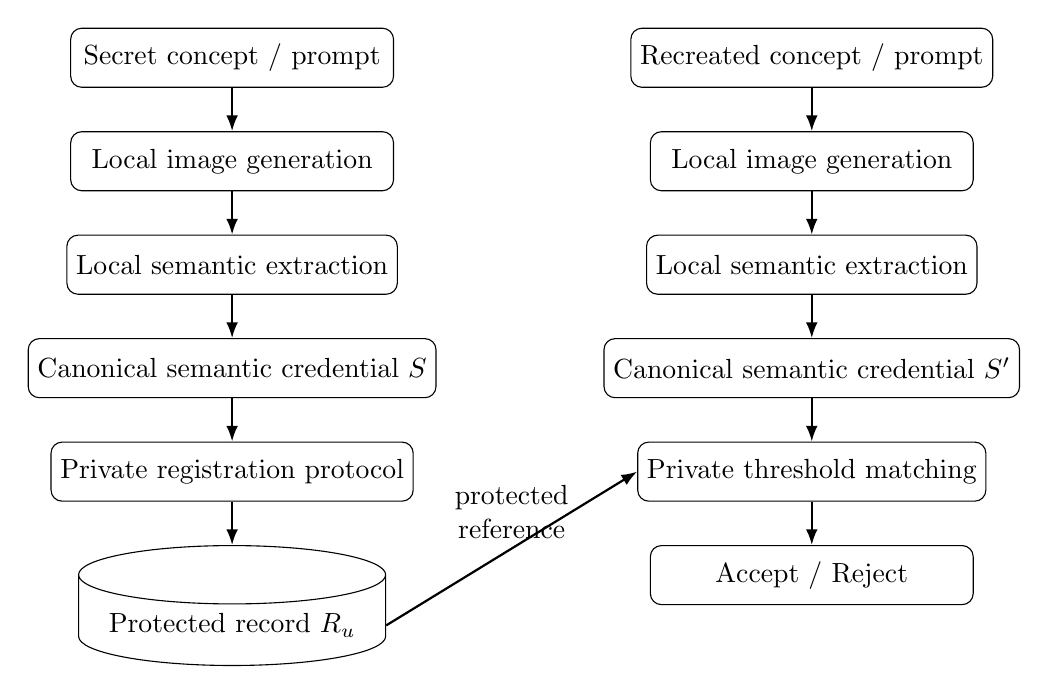
\begin{tikzpicture}[
    node distance=0.55cm and 1.5cm,
    proc/.style={rectangle,rounded corners,draw,align=center,minimum width=4.1cm,minimum height=0.75cm},
    store/.style={cylinder,shape border rotate=90,aspect=0.22,draw,align=center,minimum width=3.9cm,minimum height=0.9cm},
    arr/.style={-{Latex[length=2mm]},thick}
]
\node[proc] (p1) {Secret concept / prompt};
\node[proc,below=of p1] (g1) {Local image generation};
\node[proc,below=of g1] (e1) {Local semantic extraction};
\node[proc,below=of e1] (c1) {Canonical semantic credential $S$};
\node[proc,below=of c1] (priv1) {Private registration protocol};
\node[store,below=of priv1] (db) {Protected record $R_u$};

\node[proc,right=3.0cm of p1] (p2) {Recreated concept / prompt};
\node[proc,below=of p2] (g2) {Local image generation};
\node[proc,below=of g2] (e2) {Local semantic extraction};
\node[proc,below=of e2] (c2) {Canonical semantic credential $S'$};
\node[proc,below=of c2] (priv2) {Private threshold matching};
\node[proc,below=of priv2] (decision) {Accept / Reject};

\draw[arr] (p1)--(g1); \draw[arr] (g1)--(e1); \draw[arr] (e1)--(c1);
\draw[arr] (c1)--(priv1); \draw[arr] (priv1)--(db);
\draw[arr] (p2)--(g2); \draw[arr] (g2)--(e2); \draw[arr] (e2)--(c2);
\draw[arr] (c2)--(priv2); \draw[arr] (priv2)--(decision);
\draw[arr] (db.east) -- node[above,align=center]{protected\\reference} (priv2.west);
\end{tikzpicture}}
\caption{Target architecture. Prompt, image, and plaintext semantics remain client-side. The server stores a protected credential record and participates in a private matching protocol.}
\label{fig:architecture}
\end{figure}

The prototype should have separable modules:
\begin{enumerate}[leftmargin=*]
    \item local text-to-image generation;
    \item semantic extraction;
    \item canonicalisation/schema validation;
    \item matching engine;
    \item privacy protocol;
    \item authentication server/API;
    \item web client for demonstrator use;
    \item experiment runner;
    \item attack framework;
    \item metrics/statistical analysis; and
    \item reproducible configuration and artifact scripts.
\end{enumerate}

The research code should make it possible to run the semantic and cryptographic experiments without the web UI. The UI is a demonstrator; the experiment pipeline is the scientific artifact.

\section{Expected Contributions}

A successful paper should aim for the following contributions, subject to experimental validation:

\paragraph{C1: Formalisation of semantic credentials.}
A model of semantic visual authentication as a noisy knowledge secret with an explicit acceptance region and a security--reproducibility trade-off.

\paragraph{C2: Privacy-preserving authentication protocol.}
A concrete protocol for matching semantic credentials while minimising disclosure of the secret and reducing the value of stored authentication records to an offline attacker. The exact security claim must match the selected construction and threat model.

\paragraph{C3: AI-assisted guessing and privacy analysis.}
A systematic evaluation of frequency-based, LLM/VLM-assisted, partial-information, inversion, linkability, and adversarial-semantic attacks.

\paragraph{C4: Implementation and reproducible evaluation.}
An end-to-end prototype plus an experiment framework evaluating semantic stability, authentication accuracy, privacy leakage, attack success, model drift, and cryptographic overhead.

\section{Novelty Positioning}

The paper must not claim to be the first system that authenticates visual semantics. Closely related 2026 work already proposes image-agnostic Visual Semantic Authentication using vision-language models, explicit semantic policies, approximate matching, and hash-based secret binding. That work should be treated as a central baseline and related-work anchor.

The intended novelty is instead the combination of:
\begin{itemize}[leftmargin=*]
    \item user-reproducible generative visual concepts as noisy semantic credentials;
    \item explicit modelling of acceptance-region guessability;
    \item privacy-preserving approximate matching rather than plaintext/hash-only semantic policy evaluation;
    \item analysis of database/server compromise and cross-service linkability;
    \item AI-assisted semantic guessing based on realistic prompt distributions; and
    \item an end-to-end private authentication prototype.
\end{itemize}

If implementation or evaluation does not substantiate these differences, the paper must narrow or change its claims rather than overstating novelty.

\section{What Remains for Future Human-Subject Studies}

A later study, subject to ethics review where required, could investigate:
\begin{itemize}[leftmargin=*]
    \item whether users can remember semantic visual credentials over days or months;
    \item how people naturally construct visual-secret concepts;
    \item whether the distribution of authentication secrets differs from ordinary generative-image prompts;
    \item whether system-generated guidance can increase security without harming memorability;
    \item authentication time and error behaviour with real participants;
    \item accessibility and user-interface requirements; and
    \item comparisons with passwords, passphrases, password managers, passkeys, and graphical-password systems from a human-factors perspective.
\end{itemize}

These questions are important, but they should not be mixed into the present paper's empirical claims. The present project should establish whether the technical primitive is sufficiently secure, private, stable, and practical to justify such a study.

\section{Ethical Considerations}

The intended study avoids recruiting participants. Public datasets must be used according to their licences and documented research conditions. Even when public prompts are available, the project should minimise unnecessary retention of identifiers and should not attempt to deanonymise dataset contributors. Attack experiments should target synthetic/research accounts and locally controlled systems rather than third-party authentication services. Any newly discovered vulnerability affecting external software or services should be handled through responsible disclosure before publication.

The final PoPETs 2027 paper must use the mandatory ethical-considerations section from the official template and accurately report whether external ethics review was sought or required.

\section{Open Science and Artifact Goals}

The target artifact should enable reviewers/researchers to reproduce the principal figures and tables without manually operating the web interface. Subject to licences and storage constraints, release:
\begin{itemize}[leftmargin=*]
    \item source code;
    \item exact environment/dependency lock files;
    \item experiment configurations and random seeds;
    \item scripts to download public datasets and model weights rather than redistributing restricted content;
    \item generated non-sensitive test fixtures where licences permit;
    \item protocol benchmarks;
    \item attack scripts;
    \item analysis notebooks/scripts;
    \item raw/processed result tables needed to regenerate plots; and
    \item step-by-step artifact instructions.
\end{itemize}

The final paper must use the mandatory PoPETs 2027 Open Science section and must not promise release of materials that cannot legally or practically be distributed.

\section{Use of AI in the Research and Manuscript}

AI tools may be used for software assistance, language editing, brainstorming, or experimental components, but human authors retain responsibility for all scientific claims, references, code, experiments, and conclusions. Every bibliographic reference must be verified against the original source. Experimental prompts and model-assisted transformations that affect results must be logged and reproducible. The final PoPETs 2027 manuscript must contain the mandatory AI-use disclosure required by the venue.

\section{Working Related-Work Anchors}

The literature review should be completed systematically before claims of novelty are finalised. At minimum, the project should cover:
\begin{itemize}[leftmargin=*]
    \item graphical passwords and recognition/recall-based authentication;
    \item semantic and image-agnostic visual authentication, especially the 2026 VSA work;
    \item fuzzy extractors and secure sketches for noisy secrets;
    \item neural fuzzy extractors and privacy/security of learned authentication representations;
    \item OPRFs and threshold OPRFs;
    \item password-authenticated key exchange, including OPAQUE;
    \item PSI/PSI-cardinality and private threshold matching;
    \item homomorphic or secure-computation-based similarity matching;
    \item template protection, inversion, and linkability;
    \item AI-assisted password/credential guessing; and
    \item prompt datasets and prompt-distribution modelling, including DiffusionDB.
\end{itemize}

\paragraph{Reference hygiene.}
This research-direction document intentionally avoids pretending that an automatically generated bibliography is authoritative. Before the paper is written, all citations and BibTeX entries must be retrieved from and verified against primary sources or trusted bibliographic databases. PoPETs 2027 explicitly places responsibility for AI-assisted reference errors on the human authors.

\section{Success Criteria for the Research Direction}

The project should proceed toward a PoPETs submission only if the experiments support a coherent set of claims. A strong result would demonstrate that:
\begin{enumerate}[leftmargin=*]
    \item semantic credentials can be reproduced technically with a useful separation between intended and attacker concepts;
    \item the chosen private-matching construction substantially reduces semantic leakage or offline-verification capability relative to plaintext/hash-only baselines;
    \item the protocol has practical enough performance for an interactive authentication use case;
    \item the security analysis honestly quantifies the cost of approximate matching and low/nonuniform semantic entropy;
    \item the system remains distinguishable from existing visual-semantic authentication work through a concrete privacy contribution; and
    \item all claims can be reproduced without a human-subject experiment.
\end{enumerate}

A negative result in one dimension may still be publishable if it reveals a fundamental limitation, for example that realistic acceptance regions make semantic secrets too guessable, or that privacy-preserving matching imposes prohibitive overhead. The project should therefore optimise for scientifically defensible evidence rather than for proving the original idea correct.

\section{Conclusion}

This project investigates semantic authentication not as a claim that AI-generated images are inherently better passwords, but as a privacy problem involving noisy, nonuniform secrets. The proposed system converts independently generated images into canonical semantic credentials and uses a privacy-preserving protocol to test whether an authentication attempt falls inside the enrolled acceptance region. The research will quantify the resulting trade-offs among stability, false acceptance, false rejection, semantic guessability, stored-record privacy, linkability, and computational cost.

The principal technical challenge is to support approximate matching without turning the authentication database into a convenient semantic-guessing oracle. Structured semantic credentials combined with private set matching are the primary direction, while fuzzy-recovery/PAKE and encrypted-embedding comparison provide important alternatives and baselines. The project deliberately excludes human memorability and usability claims; those belong to future ethically reviewed user studies after the underlying privacy and security properties have been established.

\end{document}
